\documentclass{article}
\usepackage[margin=1in]{geometry}
\usepackage{graphicx}
\usepackage{xcolor}
\usepackage{float}
\usepackage{amsmath}
\usepackage{cite}
\usepackage{hyperref}
\usepackage{indentfirst}
\graphicspath{{..} {./images}}

\definecolor{navy-blue}{rgb}{0.22,0.38,0.71}

\renewcommand{\contentsname}{\vspace*{-2\baselineskip}}

\hypersetup{
	colorlinks,
	linkcolor=black,
	urlcolor=blue,
	citecolor=black
}
  		
\begin{document}
\begin{titlepage}
	\centering
	{\huge Lab 5 - Digital Modulation: Symbol Synchronization}\\[0.25 in]
	
\includegraphics[width=0.6\textwidth]{ua_logo.png}\\[0.25 in]
	{\large \textbf{ECE 531 - Software Defined Radio\\[0.25 in]
	April 4, 2025\\[0.25 in]}}
	{\large Owen Sowatzke, osowatzke@arizona.edu\\[0.05 in]
	Department of Electrical \& Computer Engineering\\[0.05 in]
	University of Arizona, Tucson, AZ 85721\\[0.5 in]}
	\hypersetup{linkcolor=navy-blue}
	\noindent\hrulefill
	\tableofcontents
	\noindent\hrulefill
\end{titlepage}

% \setlength{\parindent}{0pt}

\section{Introduction}
%Introduction to the laboratory experiment, including a brief description of the objectives and goals.

\section{Procedure}
% Detailed explanation of the laboratory experiment, including the design, implementation, and testing of the system.

\section{Results}
% Results and discussion of the laboratory experiment, including captured outputs, observations, and responses to laboratory questions.

\subsection{Pulse Shaping and Matched Filtering}

Type I Nyquist filters are defined by a rectangular pulse in the frequency domain and a sinc pulse in the time domain. The sinc pulse has zero crossings at $nT$, which produces zero ISI. Because Type I Nyquist filters are a rectangular pulse in the frequency-domain, they have the minimum bandwidth and maximize spectral efficiency. However, there are a couple problems with type I Nyquist filters. First, they are infinite in time. Second, accurate sampling is required. Small timing errors can result in large ISI because the impulse response of a sinc filter decays with $1/t$, which does not converge.

Type II Nyquist filters also have zero crossing at $nT$. However, they have a bandwidth larger than the minimum bandwidth, which allows them to achieve lower ISI sensitivity than type I Nyquist filters. The raised cosine filter is an example of a type II Nyquist filter. Its impulse responses decays with $1/t^3$, which quickly converges in the presence of timing errors.

Next, we compare the frequency response of the SRRC filters for $\beta \in [0,0.1,0.25,0.5,1]$. These frequency responses for these filters are captured in Figures \ref{fig::srrc_freq_response_beta_0} - \ref{fig::srrc_freq_response_beta_1}.

\begin{figure}[H]
	\centerline{\fbox{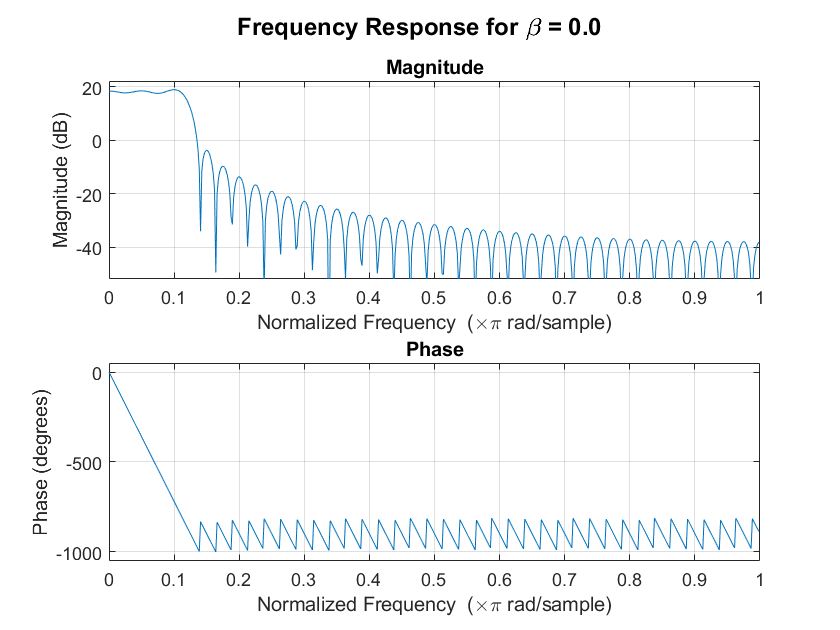
\includegraphics[width=0.5\textwidth]{srrc_freq_response_beta_0.png}}}
	\caption{SRRC Filter Frequency Response with $\beta=0$}
	\label{fig::srrc_freq_response_beta_0}
\end{figure}

\begin{figure}[H]
	\centerline{\fbox{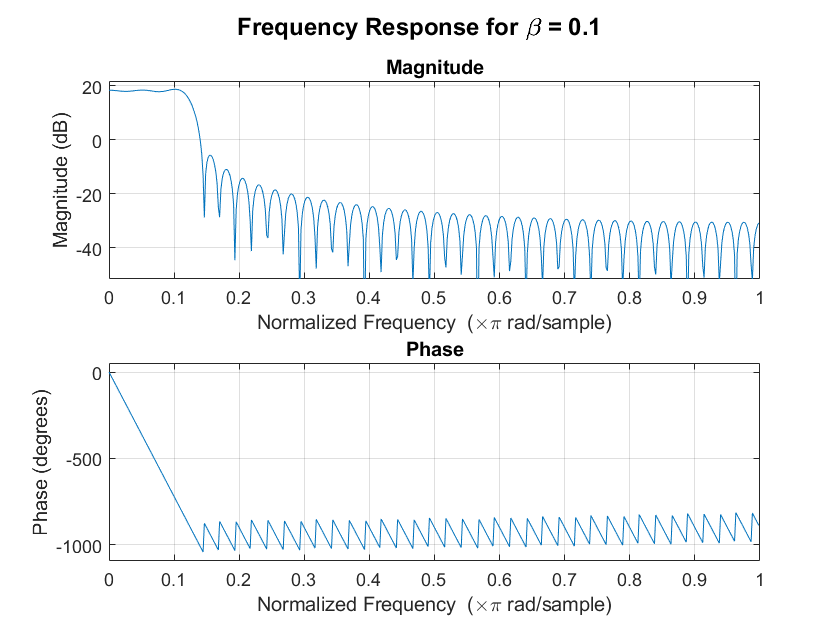
\includegraphics[width=0.5\textwidth]{srrc_freq_response_beta_0_1.png}}}
	\caption{SRRC Filter Frequency Response with $\beta=0.1$}
	\label{fig::srrc_freq_response_beta_0_1}
\end{figure}

\begin{figure}[H]
	\centerline{\fbox{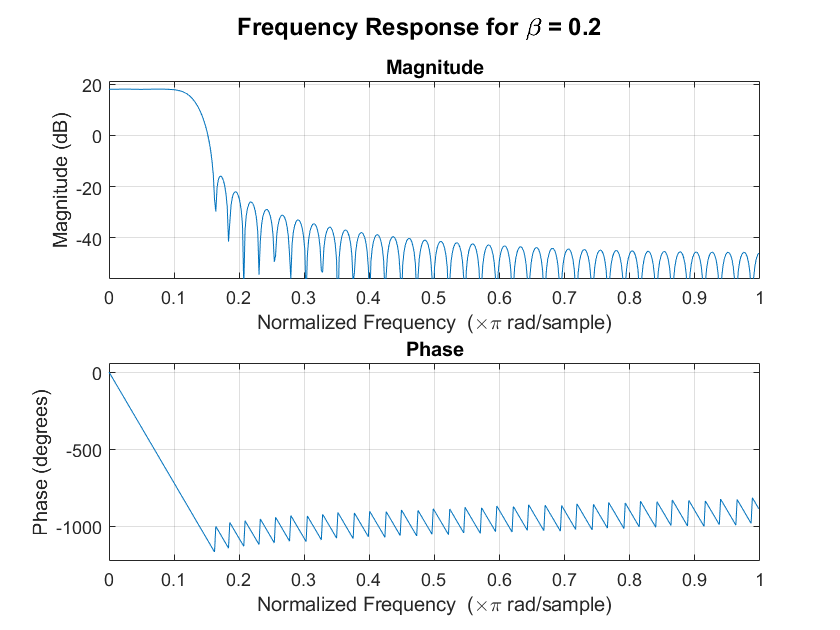
\includegraphics[width=0.5\textwidth]{srrc_freq_response_beta_0_2.png}}}
	\caption{SRRC Filter Frequency Response with $\beta=0.2$}
	\label{fig::srrc_freq_response_beta_0_2}
\end{figure}

\begin{figure}[H]
	\centerline{\fbox{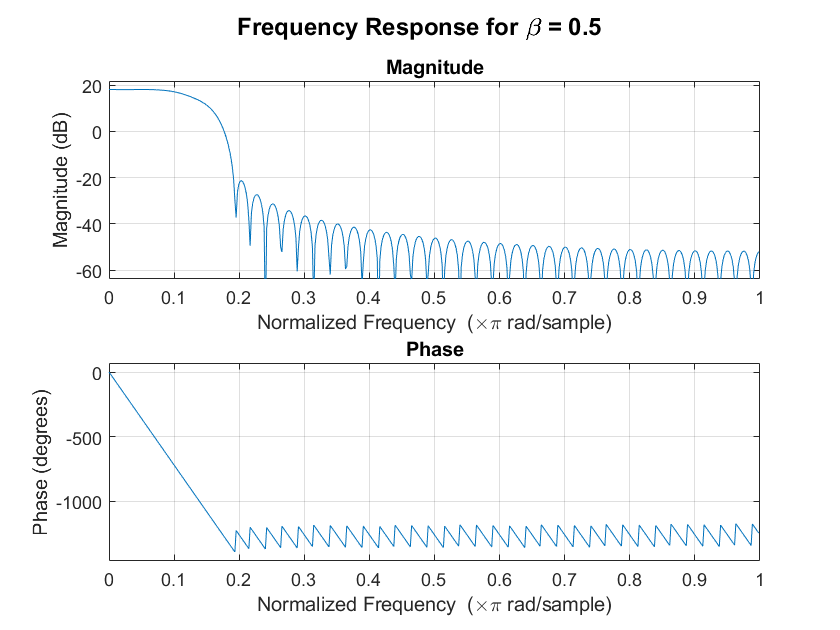
\includegraphics[width=0.5\textwidth]{srrc_freq_response_beta_0_5.png}}}
	\caption{SRRC Filter Frequency Response with $\beta=0.5$}
	\label{fig::srrc_freq_response_beta_0_5}
\end{figure}

\begin{figure}[H]
	\centerline{\fbox{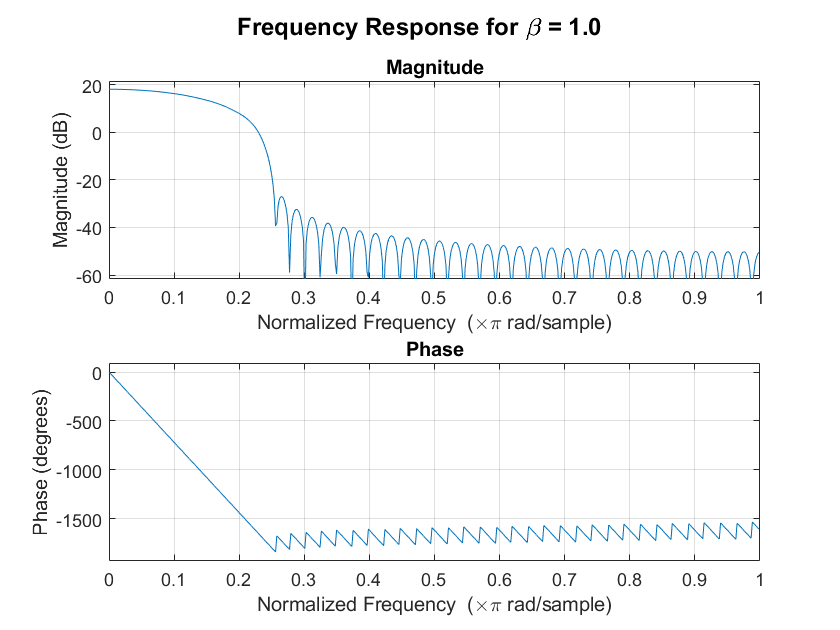
\includegraphics[width=0.5\textwidth]{srrc_freq_response_beta_1.png}}}
	\caption{SRRC Filter Frequency Response with $\beta=1$}
	\label{fig::srrc_freq_response_beta_1}
\end{figure}

\noindent Examining the frequency response of each of the filters, we see that the spectral efficiency is maximized for small values of the rolloff factor, $\beta$. However, the sharp filter transitions required for small $\beta$ increases the complexity of the filter. We can confirm this statement by plotting the impulse response of the filter with $\beta=0$ and $\beta=1$.

\begin{figure}[H]
	\centerline{\fbox{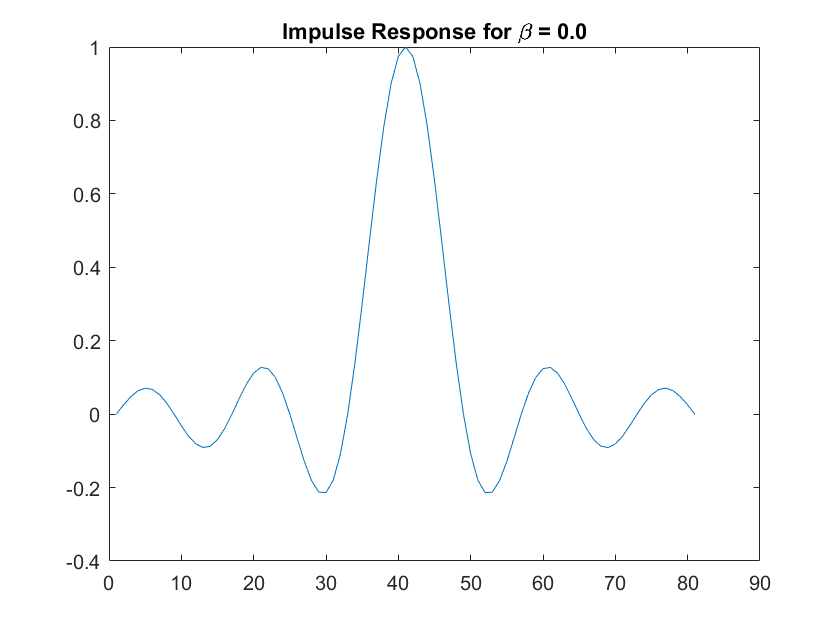
\includegraphics[width=0.5\textwidth]{srrc_impulse_response_beta_0.png}}}
	\caption{SRRC Filter Impulse Response with $\beta=0.0$}
	\label{fig::srrc_impulse_response_beta_0}
\end{figure}

\begin{figure}[H]
	\centerline{\fbox{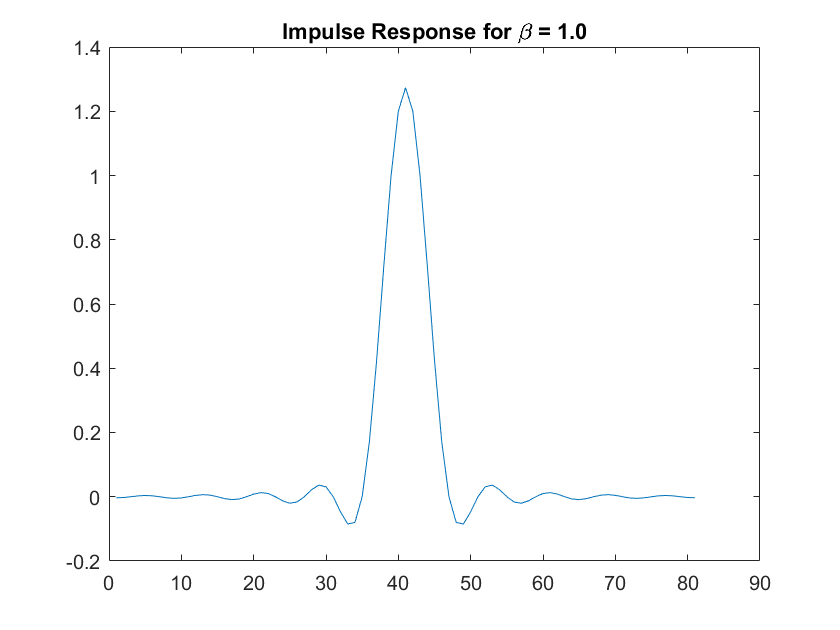
\includegraphics[width=0.5\textwidth]{srrc_impulse_response_beta_1.png}}}
	\caption{SRRC Filter Impulse Response with $\beta=1$}
	\label{fig::srrc_impulse_response_beta_1}
\end{figure}

\noindent Comparing the two impulses responses, we see that the impulse response with $\beta=1$ converges much faster than the impulse response with $\beta=0$. This allows us to truncate the impulse response sooner, which in turn reduces the filter length and complexity.

Finally, we examine how different rolloff factors affect timing recovering performance. To do this we analyze the received filter output for $\beta \in [0.1, 0.5, 0.9]$. Our results are captured in Figures \ref{fig::timing_recovery_beta_0_1} - \ref{fig::timing_recovery_beta_0_9}.

\begin{figure}[H]
	\centerline{\fbox{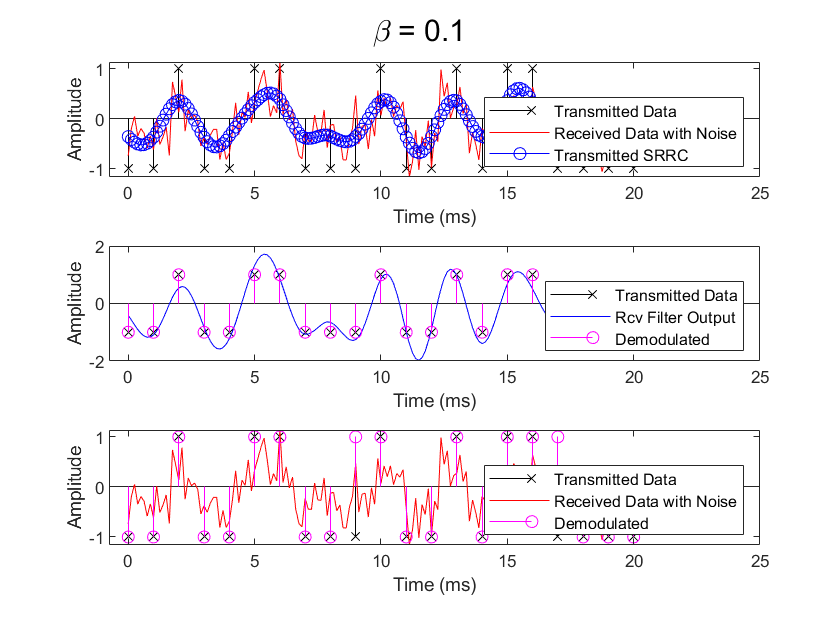
\includegraphics[width=0.5\textwidth]{timing_recovery_beta_0_1.png}}}
	\caption{Timing Recovery with $\beta=0.1$}
	\label{fig::timing_recovery_beta_0_1}
\end{figure}

\begin{figure}[H]
	\centerline{\fbox{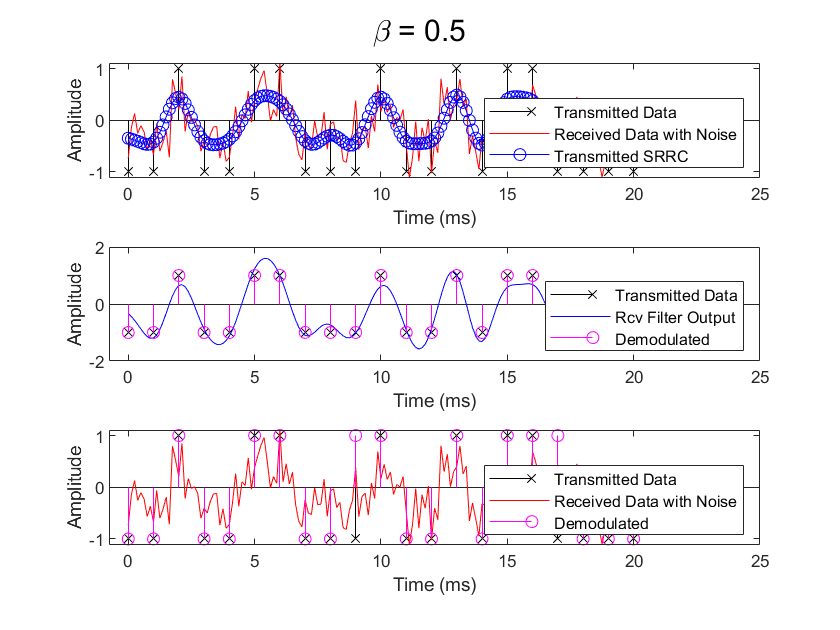
\includegraphics[width=0.5\textwidth]{timing_recovery_beta_0_5.png}}}
	\caption{Timing Recovery with $\beta=0.5$}
	\label{fig::timing_recovery_beta_0_5}
\end{figure}

\begin{figure}[H]
	\centerline{\fbox{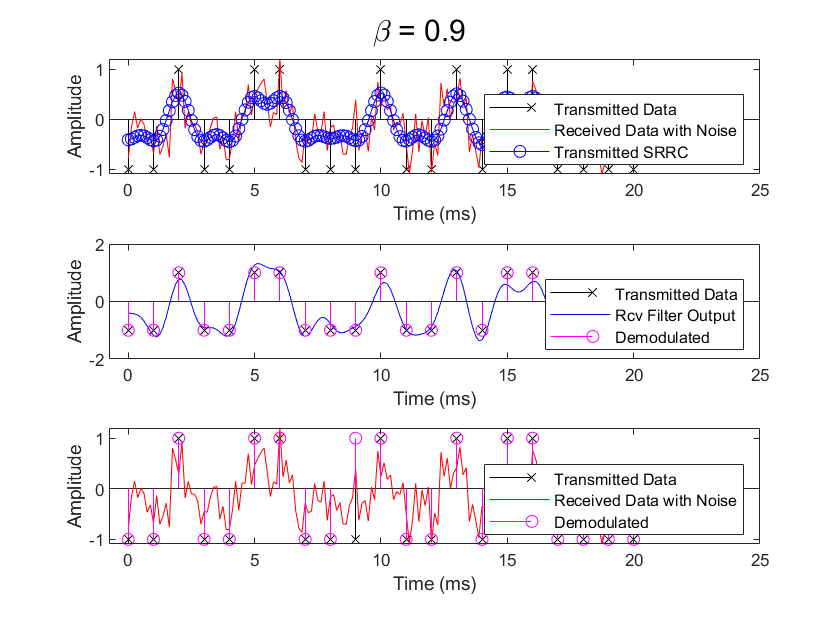
\includegraphics[width=0.5\textwidth]{timing_recovery_beta_0_9.png}}}
	\caption{Timing Recovery with $\beta=0.9$}
	\label{fig::timing_recovery_beta_0_9}
\end{figure}

\noindent The received filter outputs (shown in solid blue) allow us to visualize the effect of various timing offsets. For small values of $\beta$, the receive filter output overshoots the demodulated points more than it does for large values of $\beta$. Given a small timing offset, smaller values of $\beta$ will result in greater timing errors.

\subsection{Timing Error}

In this section, we capture a QPSK constellation with the PlutoSDR. Our captured constellation is shown in Figure \ref{fig::pluto_constellation_raw}.

\begin{figure}[H]
	\centerline{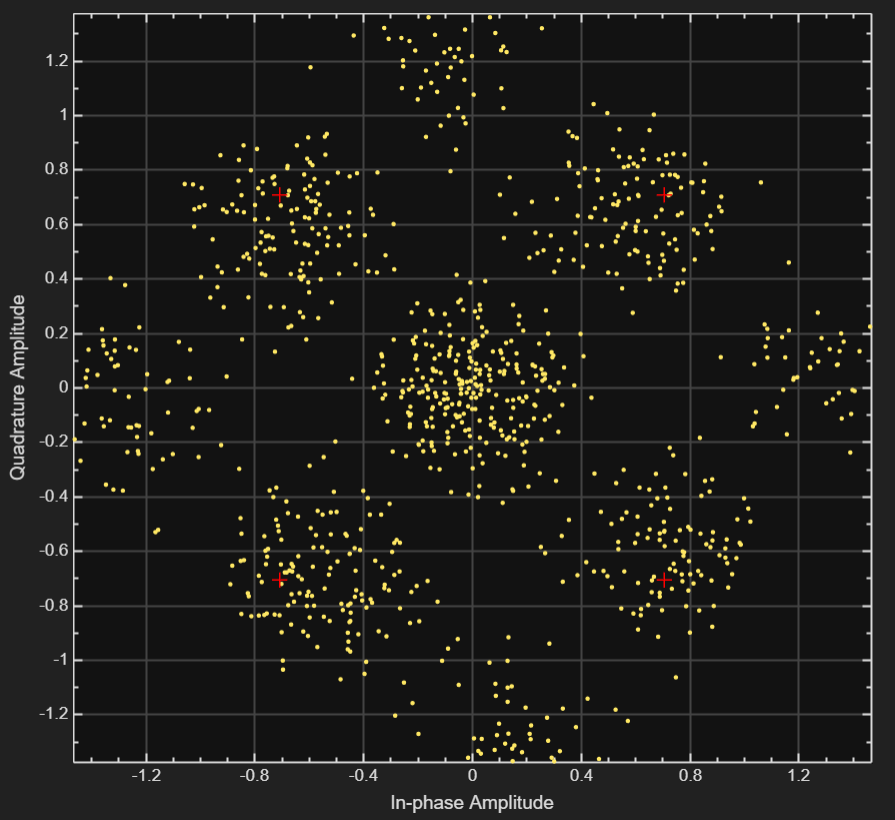
\includegraphics[width=0.5\textwidth]{pluto_constellation_raw.png}}
	\caption{QPSK Constellation Captured with Pluto SDR}
	\label{fig::pluto_constellation_raw}
\end{figure}

\noindent We also leverage code from \texttt{plutoLoopback.m} to sweep timing offsets. If we sweep the timing offsets, we can perform a manual timing compensation. With the best timing compensation, we get the constellation shown in Figure \ref{fig::pluto_constellation_best}.

\begin{figure}[H]
	\centerline{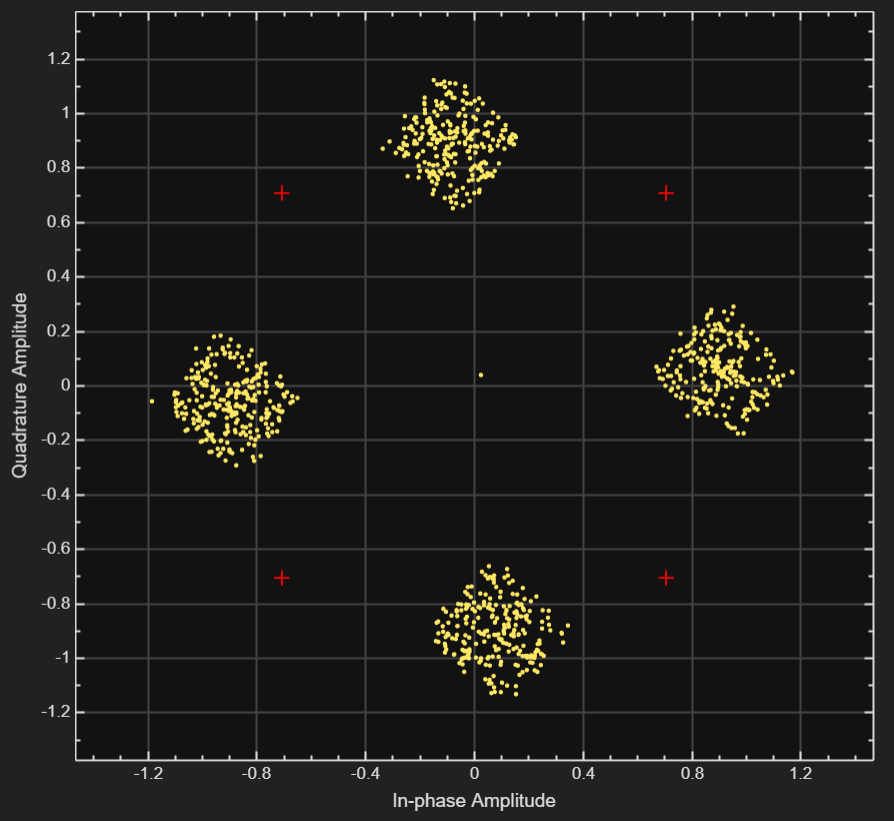
\includegraphics[width=0.5\textwidth]{pluto_constellation_best.png}}
	\caption{QPSK Constellation After Manual Timing Compensation}
	\label{fig::pluto_constellation_best}
\end{figure}

\noindent Before timing compensation, the signal is sampled at non-ideal points, resulting in increased constellation point errors. These increased errors create large clustering patterns in the constellation. After correcting for these timing errors, the errors in the constellation are reduced. However, our constellation remains titled. This titled occurs due to a phase offset in the transmit and receive oscillators. Regardless of what we do with the timing compensation, this phase offset will still be present.

\section{Symbol Timing Compensation}

In this section, we perform symbol timing compensation in MATLAB. To do this, we implement two custom MATLAB implementations, which we benchmark against MATLAB's \texttt{comm.SymbolSynchronizer}. For the first implementation, we connect the textbook-provided routines together following the structure shown in Figure \ref{fig::timing_recovery_block_diagram}.

\begin{figure}[H]
	\centerline{\fbox{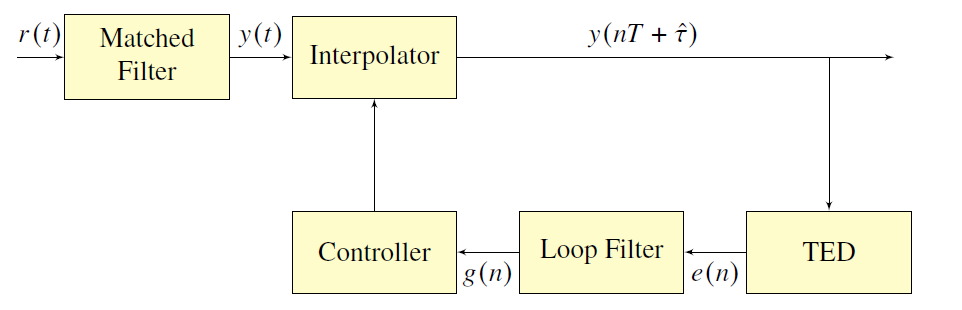
\includegraphics[width=0.7\textwidth]{timing_recovery_block_diagram.png}}}
	\caption{Structure of Timing Recovery PLL}
	\label{fig::timing_recovery_block_diagram}
\end{figure}

\noindent For the second implementation, we create custom system objects for each of the blocks in the timing recovery PLL and then connect them in the appropriate manner. In each implementation, we use a zero-crossing (ZC) timing detector and the following loop filter parameters:

\begin{equation*}
	[N, \zeta, B_{loop}, G_D] = [2, 1, 0.01, 2.7]
\end{equation*}

\noindent To characterize our timing recovery circuits, we create noise-free data with a fixed timing error. We then run the custom implementations and MATLAB's \texttt{comm.SymbolSynchronizer} on the same generated data. In Figure \ref{fig::symbol_sync_no_noise} and \ref{fig::fractional_error_no_noise}, we plot the synchronized symbols and the fractional delay ($\mu(n)$) output by each routine on the same axes.

\begin{figure}[H]
	\centerline{\fbox{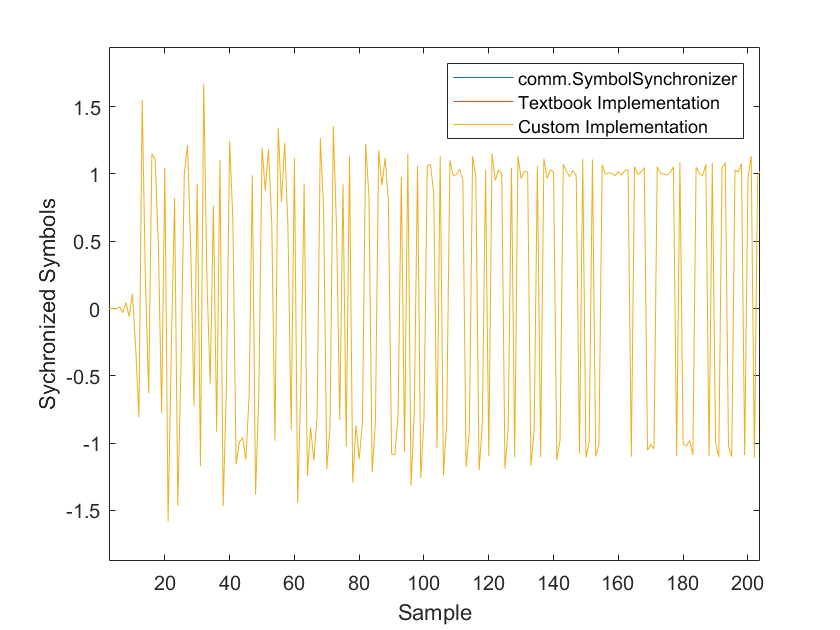
\includegraphics[width=0.5\textwidth]{symbol_sync_no_noise.png}}}
	\caption{Comparison of Synchronized Symbols}
	\label{fig::symbol_sync_no_noise}
\end{figure}

\begin{figure}[H]
	\centerline{\fbox{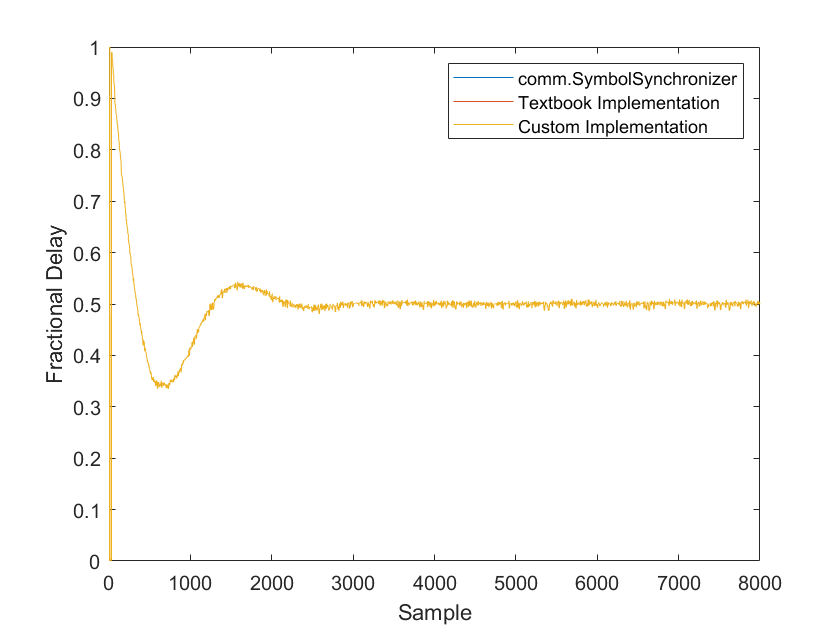
\includegraphics[width=0.5\textwidth]{fractional_error_no_noise.png}}}
	\caption{Comparison of Fractional Error}
	\label{fig::fractional_error_no_noise}
\end{figure}

\noindent Comparing the outputs of each routine, we see that the routine outputs are approximately the same, indicating a correct implementation. We also see that the loop filter parameters cause the fractional delay to converge. For completeness, we also plot the error between the \texttt{comm.SymbolSynchronizer} outputs and the custom routine outputs. 

  first implementation we create from the textbook-provided scripts

. For our timing compensation, we  timing error correction in MATLAB. We do this in this in two 
\section{Conclusion}
% Conclusions to the overall lab that discuss meaningful lessons learned and other takeaways from the assignment. (Important)
	
\end{document}